\newpage
\section{Variationen des Graphen}
Die Aufgabenstellung legt die Topologie des planaren Graphen\footnote{Ein planarer Graph hat die Eigenschaft, dass er in der 2. Dimension dargestellt werden kann, ohne dass sich seine Kanten überschneiden.} fest, auf dem sich das Fahrzeug bewegen soll. Diese bleibt abgesehen von fehlenden Kanten oder blockierten Knotenpunkten fest. In einer 2D Darstellung können die Knotenpunkte in dem Rahmen verschoben werden, sodass die Topologie nicht verletzt wird. Das Ziel ist es, eine robuste Simulation zu erstellen, die mit möglichst vielen unterschiedlichen Variationen des Graphen funktioniert. Dafür wurde ein Tool entwickelt, das anhand eines Start-Graphen valide Variationen desselben entdeckt und diese abspeichert. Die erstellten Graphen können für den Simulator, sowie die virtu

\begin{figure}[h!]
            \centering
            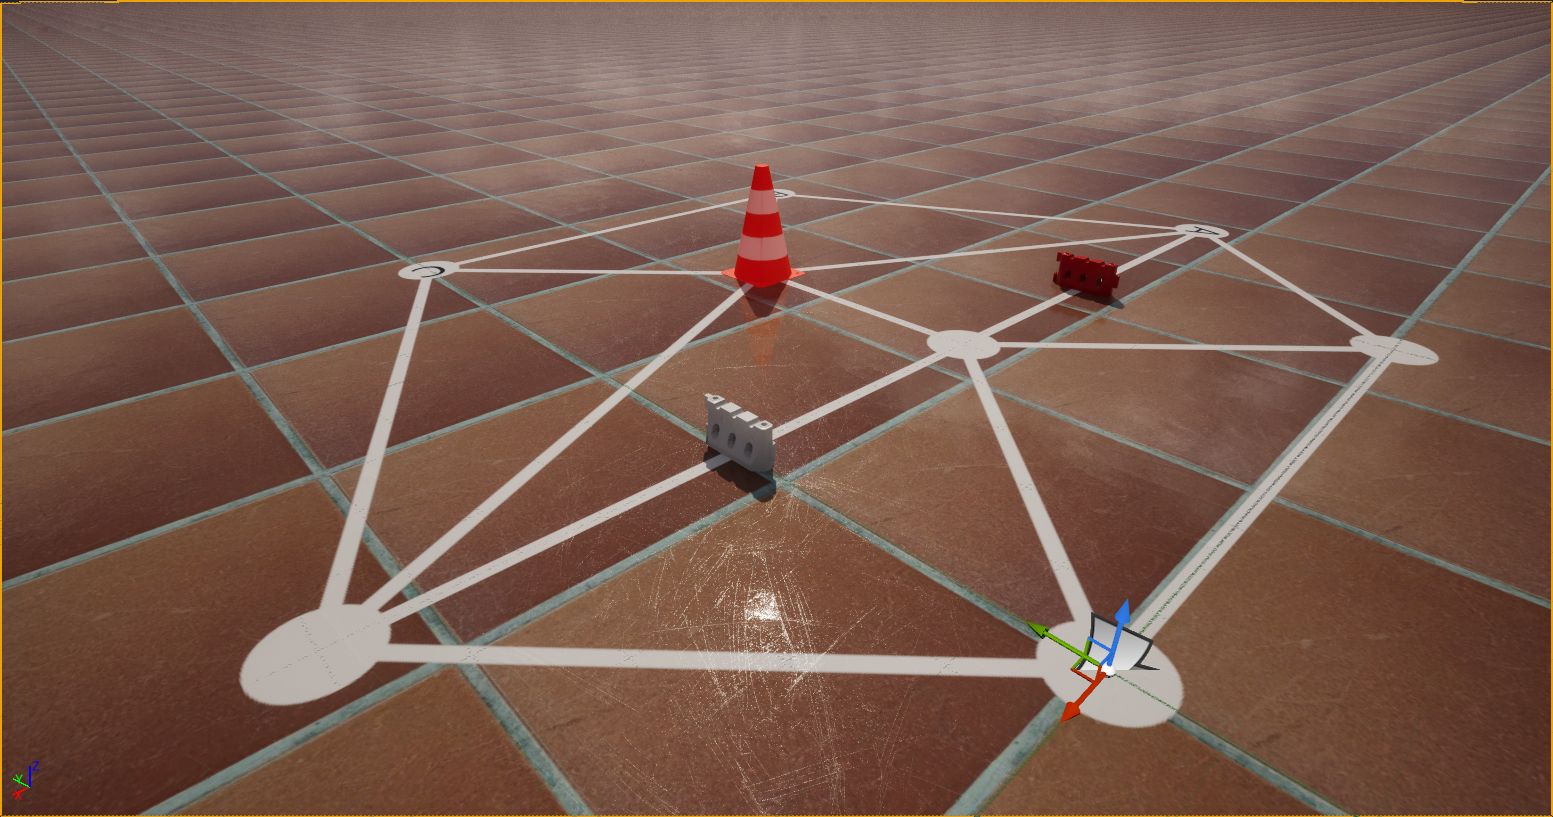
\includegraphics[width=0.9\textwidth]{img/unrealengine/overview.png}
            \caption{Übersicht Unreal Engine}
        \label{img:Übersicht Unreal Engine}
        \end{figure}
\subsection{Kamera-Konfiguration}
Unreal Engine erlaubt das einfache Testen von verschiedenen Kamera-Konfigurationen. Unter anderem Das Kamera-Sichtfeld, sowie verschiedene Neigungswinkel. In folgender Tabelle sind die Ergebnisse unterschiedlicher Kamerakonfigurationen zu sehen. Dabei stellt der grüne Kreis eine horizontale Distanz von 4.5m von der Kamera entfernt, und der weisse Kreis eine horizontale Distanz von 2m von der Kamera entfernt dar.